\documentclass[10pt]{article}

\usepackage[paperwidth=18cm, paperheight=11.5cm, margin=0cm]{geometry}
\usepackage{graphicx}
\hyphenpenalty=10000

\begin{document}

\centering

\noindent
\raisebox{5cm}{\textsf{A}}
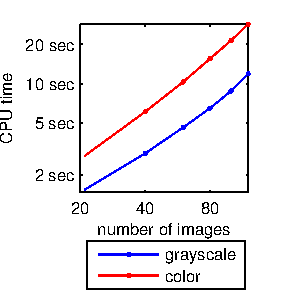
\includegraphics[width=5.5cm]{timing_studies_nimages}
%
\raisebox{5cm}{\textsf{B}}
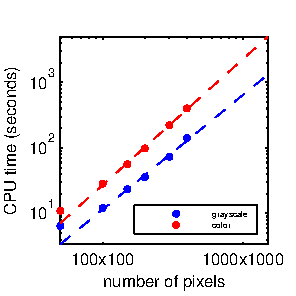
\includegraphics[width=5.5cm]{timing_studies_npixels}
%
\raisebox{5cm}{\textsf{C}}
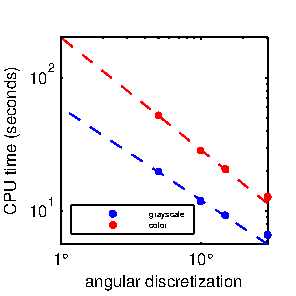
\includegraphics[width=5.5cm]{timing_studies_nrot}

\noindent
\raisebox{2.5cm}{\textsf{D}}
{\renewcommand{\arraystretch}{1.5}
{ \textsf{ \small
\begin{tabular}{ | p{2cm} | c | c | c | c | c | c | }
\hline
Data Set &
Data Type &
\parbox[c]{2cm}{ \centering Number of Channels} &
\parbox[c]{2cm}{ \centering \vspace{.5\baselineskip} Number of Images \vspace{.5\baselineskip}} &
\parbox[c]{2cm}{ \centering Number of Pixels} &
\parbox[c]{2cm}{ \centering Angular Discretization} &
\parbox[c]{2cm}{ \centering CPU time}  \\
\hline
{\em Drosophila} gastrulation (live) & 2D & 1 & 40 & 100 $\times$ 100 & 10$^\circ$ & 3.2~sec \\
Zebrafish epiboly & 2D & 1 & 120 & 100 $\times$ 100 & 10$^\circ$ & 13~sec\\
{\em Drosophila} gastrulation (fixed) & 2D & 3 & 120 & 100 $\times$ 100 & 10$^\circ$ & 29~sec  \\
{\em Drosophila} wing discs & 3D & 3 & 46 & 100 $\times$ 100 $\times$ 21 & 10$^\circ$ & 12~sec  \\
 \hline
\end{tabular}}}}

\end{document}